\clearpage
\paragraph{LoRa}
\verb|LoRa from "Long Range"| is a radio communication technology that is designed with long range in mind.

The telemetry system uses a \verb|LoRa| module to transmit data from the vehicle to the pit crew.
This allows the team to monitor the vehicle's performance in real time and make informed decisions during
the race.

The device shows up on \verb|Linux| as a \verb|tty| device. For parsing purposes a simple frame structure was designed.
Each packet has the structure \texttt{[0xFF][data][0xEE]}, where \texttt{0xFF} is the start byte and \texttt{0xEE} is the end byte.
After this frame the \verb|LoRa| module needs to receive the sequence \texttt{\textbackslash{}n\textbackslash{}r} to send the packet.\\

To initialize this peripheral, the serial port needs to be configured in the following way:
\begin{figure}[!htb]
    \centering
    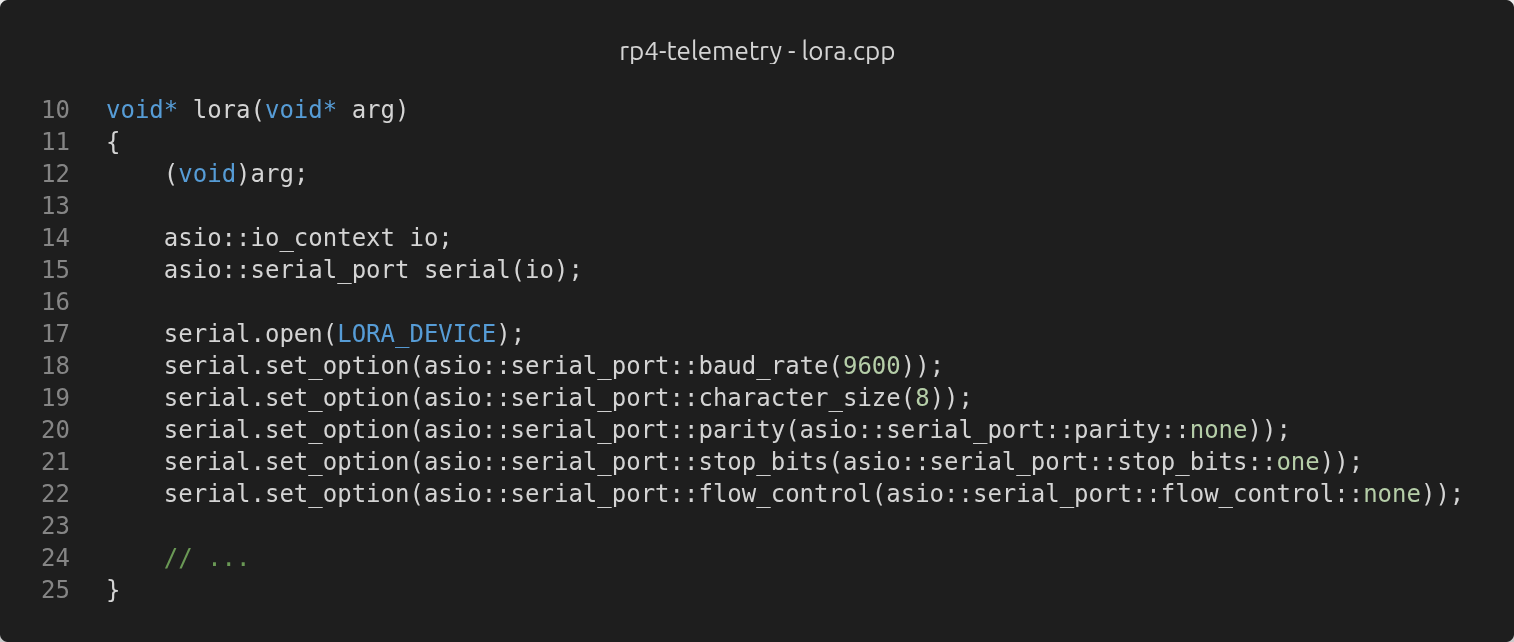
\includegraphics[width=0.9\textwidth]{images/code/lora_init.png}\par
    \caption{Initializing the LoRa module}
    \label{fig:code-lora-init}
\end{figure}
\FloatBarrier

The main data sending loop is structured in the following way:
\begin{figure}[!htb]
    \centering
    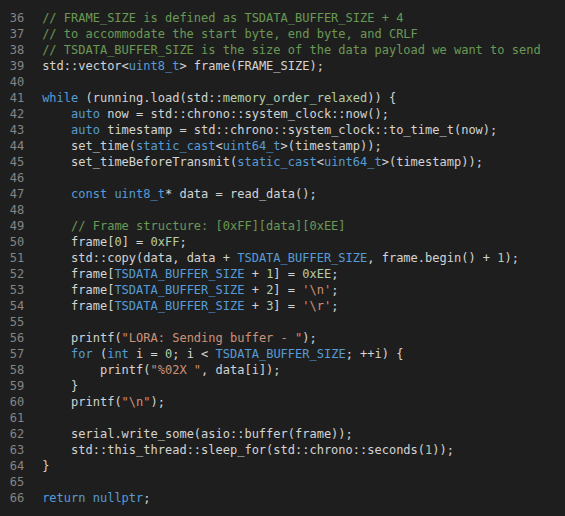
\includegraphics[width=0.7\textwidth]{images/code/lora_send.png}\par
    \caption{Main LoRa sending loop}
    \label{fig:code-lora-send}
\end{figure}
\FloatBarrier